\documentclass[../../main.tex]{subfiles}

%-----------------------------------------------------------%
\begin{document}
\section{Configurational Layout}
\begin{enumerate}
    \item \textbf{Software:} SolidWorks 2019 is used for modelling
    \item \textbf{Model name:} STD0010002
    \begin{figure}[H]
        \centering
        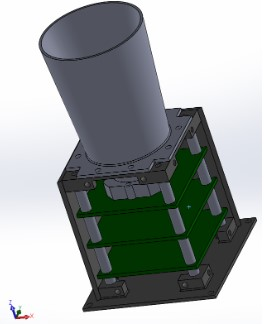
\includegraphics{Figures/Mechanical/stads_full.jpg}
        \caption{STADS CAD Model}
        \label{fig:sys_CAD}
    \end{figure}
    \text need to include labelled exploded view for STADS CAD.
    \item \textbf{Axes of the system:} + Z Axis - Opposite to the outward normal of face connected to optical system (Top panel outward normal).
    \item \textbf{Components to be incorporated into STADS:} Optics components not included
    \begin{table}[h!]
        \centering
        \begin{tabular}{| p{5cm} | p{3cm} |}
             \hline
             \textbf{Component Name} & \textbf{Quantity}  \\
             \hline
             PCB & 3 \\
             \hline
             Side Panels & 4 \\
             \hline
             Top Panel & 1 \\
             \hline
             Bottom Panel & 1 \\
             \hline
             Solid Rods & 4 \\
             \hline
             Spacers & 16 \\
             \hline
        \end{tabular}
        \caption{Components}
        \label{tab:my_label}
    \end{table}
    \item The STADS module is broken down into stacked components and face mounted components.
    \begin{enumerate}
        \item \textbf{Stacked Components:} All PCBs are stacked inside STADS using solid rods and spacers.
        \text include image here %%%%%%%%%%%%%%%%%
        \begin{enumerate}
            \item 4 solid rods run through all the PCBs symmetrically. Spacers are used to keep PCBs and Panels vertically distant as required.
            \text here is an image
            \item The Optical system is broken down into components placed on PCB and Baffle. Here component on PCB and PCB itself is stacked using spacers and solid rod.
            \text here there is an image
        \end{enumerate}
    \end{enumerate}
    \item \textbf{Face mounted:} Face mounted components include Side Panels and 
    Baffle. The Baffle is directly connected to the Top Panel using 8 screws.
    \begin{enumerate}
        \item There is an image here
        \item  Again we have a image
        \item The caption  to the above image is: The Bottom Panel acts as a mechanical interface to the user satellite and interfacing Side panels. It also act as a starting block for stacking of PCBs.
        \item image
        \item here's another caption: \textbf{Side Panels on the 4 side in X and Y axis have 2 purposes of doing radiation shielding and structural stability. Further modification of incorporating connector in our system can be done on these.}
    \end{enumerate}
    \item \textbf{Parallel Configuration}:
    \begin{enumerate}
        \item \textbf{Stacking with support rail:} In this configuration stacking of PCB is done using stubs present on support rails. Also the interface of all panels is done to these support rails.
        \item Here we have an image of the stack,
        \item \textbf{Top Panel with Extruded Stubs:} In this configuration mechanical interfacing with user satellite is done using Extruded Stubs present on Top panel.
        \item Here we have two images side-to-side.
    \end{enumerate}
\end{enumerate}
%----------------------------END----------------------------%
\end{document}